\chapter{Cruscotto di controllo della qualità} \label{sec:cruscotto}

\section{Varianza dell'impegno orario}
\begin{figure}[H]
    \centering
    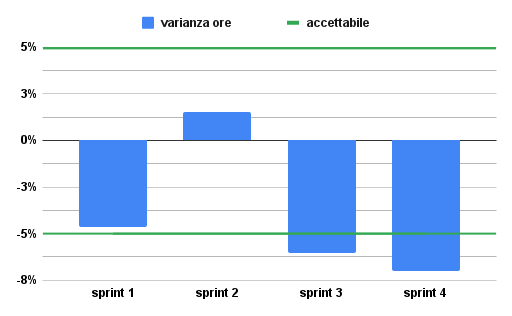
\includegraphics[width=0.8\linewidth]{VarOre.png}
    \caption{Varianza dell'impegno orario per sprint}
\end{figure}
\subsection{Analisi}
Analizzando i valori riportati nel grafico, è riscontrabile una difficoltà nel produrre preventivi orari vicini al consuntivato.\\
In particolare, vengono registrati dei valori di poco inferiori all'accettabile nel terzo e quarto sprint e un valore di poco superiore nel quinto sprint. Il motivo del numero inferiore o superiore di ore produttive è stato esaminato nell'analisi retrospettiva presente nel Piano\_di\_progetto\_v1.0.

\section{Varianza di Budget}
\begin{figure}[H]
    \centering
    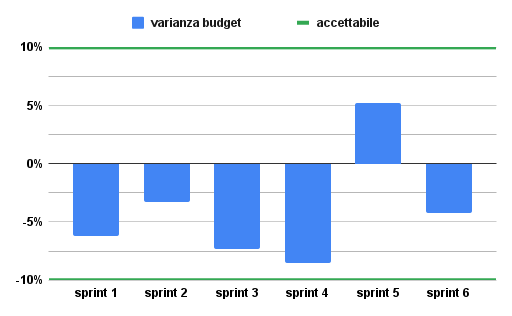
\includegraphics[width=0.8\linewidth]{VarBud.png}
    \caption{Varianza di Budget per sprint}
\end{figure}
\subsection{Analisi}
Dall'analisi del grafico è immediato osservare che i valori di varianza di budget sono sempre rimasti all'interno della soglia di accettabilità.\\
Il risultato evidenziato è tuttavia migliorabile: sebbene non sia mai stato speso più del preventivato in uno sprint, è importante in futuro migliorare la fase di pianificazione. L'obiettivo deve essere quello di definire preventivi sempre più realistici, partendo da quanto consuntivato negli sprint precendenti, impegnandosi a utilizzare le ore e le risorse stanziate.

\section{Estimate to Complete e Estimate at Completion}
\begin{figure}[H]
    \centering
    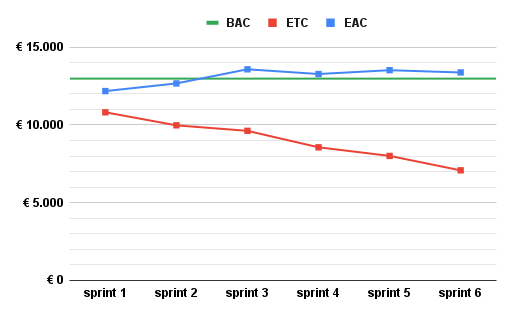
\includegraphics[width=0.8\linewidth]{ETCEAC.png}
    \caption{Progressione Estimate to Complete e Estimate at Completion in relazione al Budget at Completion}
\end{figure}
\subsection{Analisi}
Dopo un ottimo inizio nei primi due sprint, è possibile notare un calo dei lavori nel terzo sprint, e un altro leggero rallentamento nel quinto. L'Estimate to Complete al terzo e al quinto sprint è diminuito in modo meno marcato rispetto lo sprint precedente. Inoltre, l'Estimate at Completion ha superato il Budget at Completion.\\
Questo è causato dal mancato raggiungimento di tutti gli obiettivi fissati dalla milestone del terzo sprint. Il valore dopo il terzo sprint è rimasto stabile ad un valore poco al di sopra del Budget at Completion.

\section{Planned Value, Earned Value e Actual Cost}
\begin{figure}[H]
    \centering
    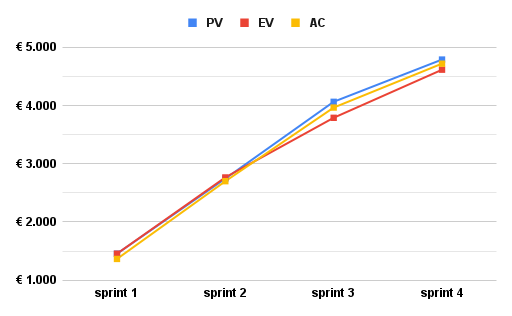
\includegraphics[width=0.8\linewidth]{PVEVAC.png}
    \caption{Progressione Planned Value, Earned Value e Actual Cost}
\end{figure}
\subsection{Analisi}
Dopo un ottimo inizio nei primi due sprint, come in altre metriche è possibile notare un calo dei lavori nel terzo. Se fino al secondo sprint i valori di Planned Value, Earned Value e Actual Cost erano quasi identici, a terzo sprint completato è riscontrabile dal cruscotto il "distaccamento" dei tre valori.\\
Questo è causato dal mancato raggiungimento di tutti gli obiettivi fissati dalla milestone del terzo sprint, che hanno portato l'Earned Value ad essere minore del Planned.

\section{Schedule Variance e Cost Variance}
\begin{figure}[H]
    \centering
    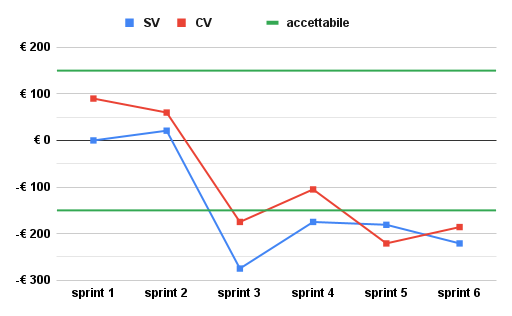
\includegraphics[width=0.8\linewidth]{SVCV.png}
    \caption{Progressione Schedule Variance e Cost Variance}
\end{figure}
\subsection{Analisi}
Dopo un ottimo inizio nei primi due sprint, come in altre metriche è possibile notare un calo dei lavori nel terzo. Se fino al secondo sprint i valori di Schedule e Cost Variance mostravano un anticipo sui lavori rispetto il costo preventivato per eseguirli, il mancato raggiungimento di tutti gli obiettivi fissati dalla milestone del terzo sprint ha portato a dei valori negativi. Dal quarto sprint in poi i valori sono aumentati riportandosi e stabilendosi ad un livello di poco inferiore all'accettabile. Nel quinto sprint è riscontrabile un calo dei lavori dovuto al periodo di vacanze, il quale però era stato previsto.

\section{Schedule Performance Index e Cost Performance Index}
\begin{figure}[H]
    \centering
    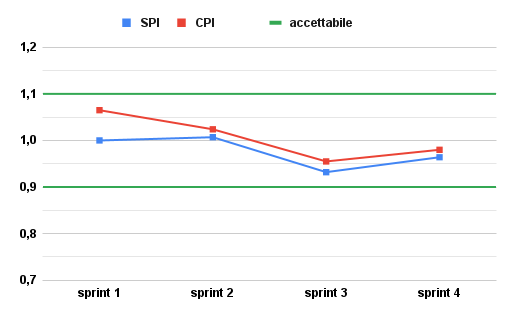
\includegraphics[width=0.8\linewidth]{SPICPI.png}
    \caption{Progressione Schedule Performance Index e Cost Performance Index}
\end{figure}
\subsection{Analisi}
Similmente a quanto riscontrabile dall'analisi dei valori di Schedule e Cost Variance, i valori di Schedule Performance Index e Cost Performance Index sono scesi sotto l'1 con la fine dello sprint 3. I valori comunque rimangono ampiamente all'interno dei valori accettabili stabilendosi sullo 0,97.

\section{Misure di mitigazione insufficienti}
\begin{figure}[H]
    \centering
    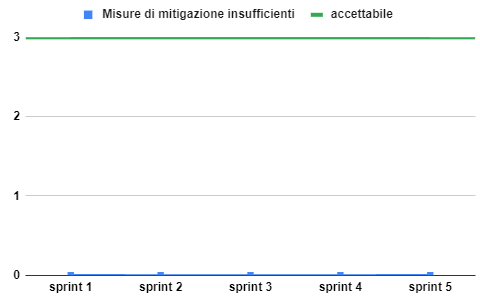
\includegraphics[width=0.8\linewidth]{Mitigazioni.png}
    \caption{Progressione occorrenza di rischi con misure mitigative insufficienti}
\end{figure}
\subsection{Analisi}
Come riscontrabile dai valori riportati dal grafico, l'ampia analisi dei rischi effettuata a inizio progetto ha portato alla definizione di misure mitigative che hanno sempre avuto efficacia.

\section{Rischi inattesi}
\begin{figure}[H]
    \centering
    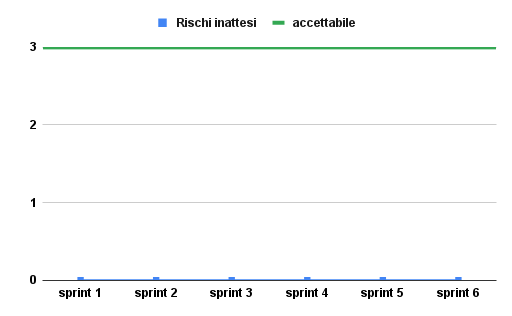
\includegraphics[width=0.8\linewidth]{Rischi.png}
    \caption{Progressione occorrenza di rischi inattesi}
\end{figure}
\subsection{Analisi}
Come riscontrabile dai valori riportati dal grafico, l'ampia analisi dei rischi effettuata a inizio progetto ha portato alla definizione di molti rischi riscontrabili. In particolare, nessun rischio riscontrato fino ad ora non era stato preventivato per tempo.

\section{Requisiti soddisfatti}
\begin{figure}[H]
    \centering
    \begin{minipage}[b]{0.32\textwidth}
        \centering
        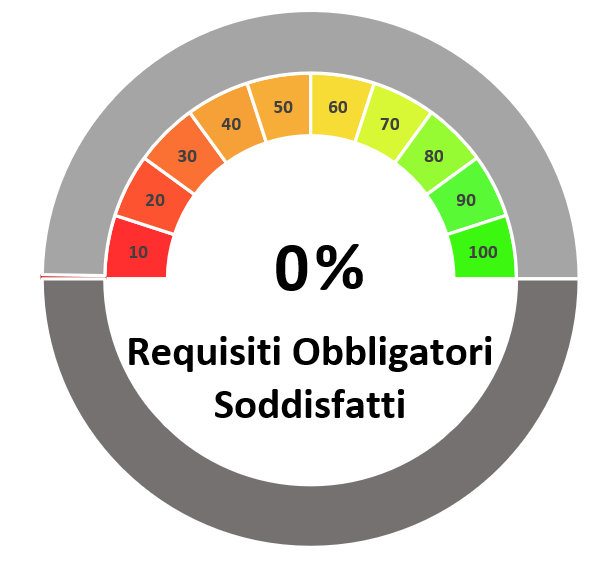
\includegraphics[width=\textwidth]{ReqObbSodd.png}
        \caption{Requisiti obbligatori soddisfatti}
        \label{reqobbsodd}
    \end{minipage}
    \hfill
    \begin{minipage}[b]{0.32\textwidth}
        \centering
        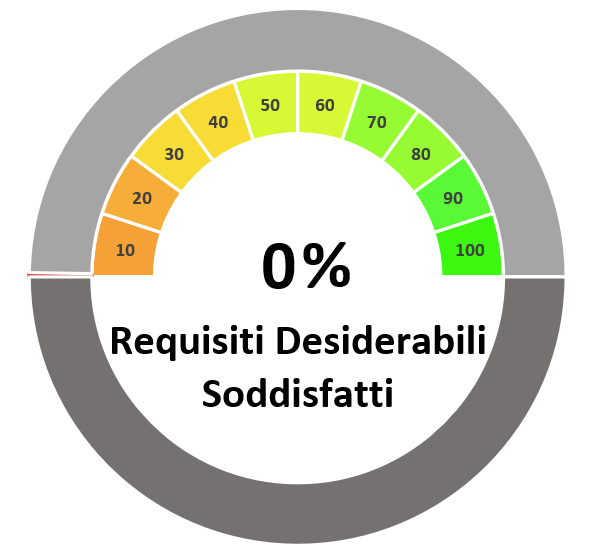
\includegraphics[width=\textwidth]{ReqDesSodd.png}
        \caption{Requisiti desiderabili soddisfatti}
        \label{reqdessodd}
    \end{minipage}
    \hfill
    \begin{minipage}[b]{0.32\textwidth}
        \centering
        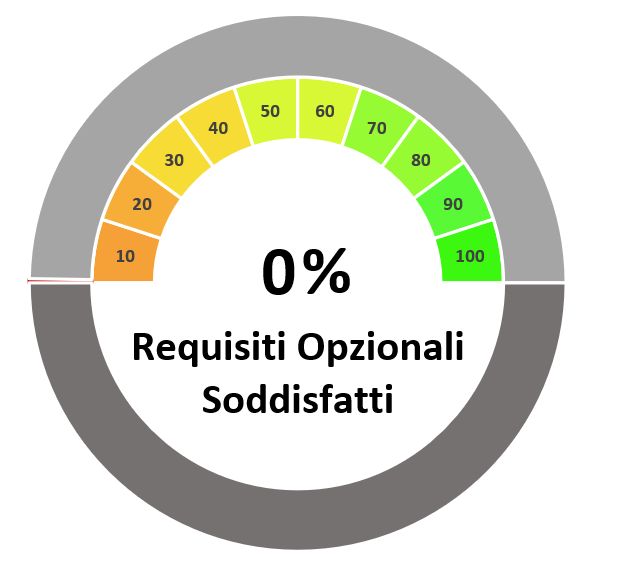
\includegraphics[width=\textwidth]{ReqOpzSodd.png}
        \caption{Requisiti opzionali soddisfatti}
        \label{reqopzsodd}
    \end{minipage}
\end{figure}
\subsection{Analisi}
Il progetto fino ad ora ha prodotto un Proof of Concept, dunque nessun prodotto finale con il quale soddisfare alcun requisito.\\Per questo motivo è normale che nel cruscotto non risulti soddisfatto nessun requisito.

\section{Indice di Gulpease}
\begin{figure}[H]
    \centering
    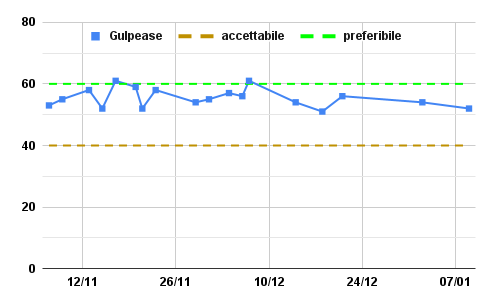
\includegraphics[width=0.8\linewidth]{GulpeaseVerbaliProgresso.png}
    \caption{Progressione indice di Gulpease dei verbali}
\end{figure}
\begin{figure}[H]
    \centering
    \begin{minipage}[b]{0.45\textwidth}
        \centering
        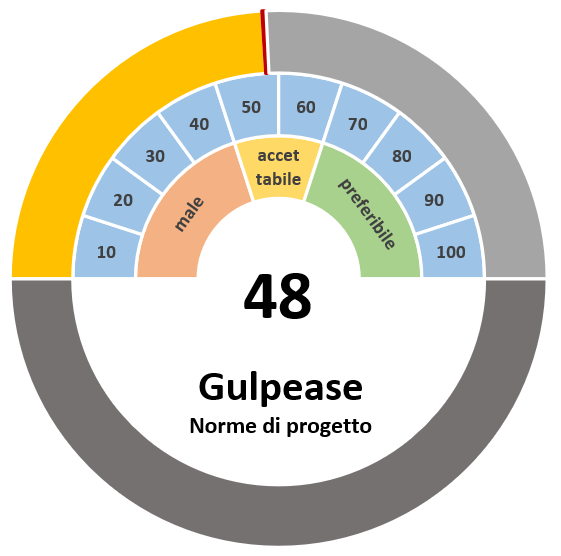
\includegraphics[width=\textwidth]{GulpeaseNdp.png}
        \caption{Gulpease di Norme\_di\_progetto\_v1.0}
    \end{minipage}
    \hfill
    \begin{minipage}[b]{0.45\textwidth}
        \centering
        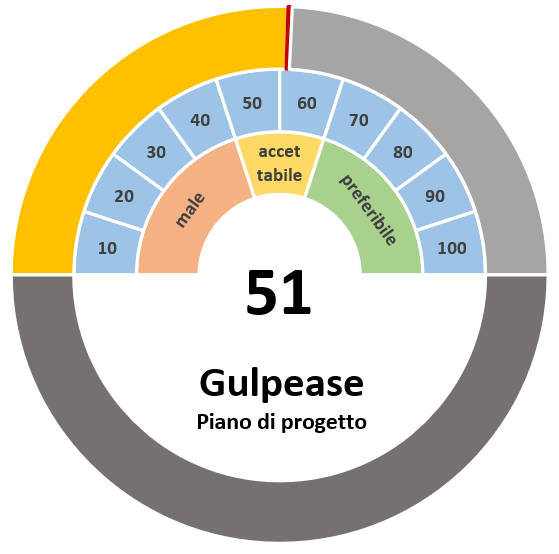
\includegraphics[width=\textwidth]{GulpeasePdp.png}
        \caption{Gulpease di Piano\_di\_progetto\_v1.0}
    \end{minipage}
\end{figure}
\begin{figure}[H]
    \centering
    \begin{minipage}[b]{0.45\textwidth}
        \centering
        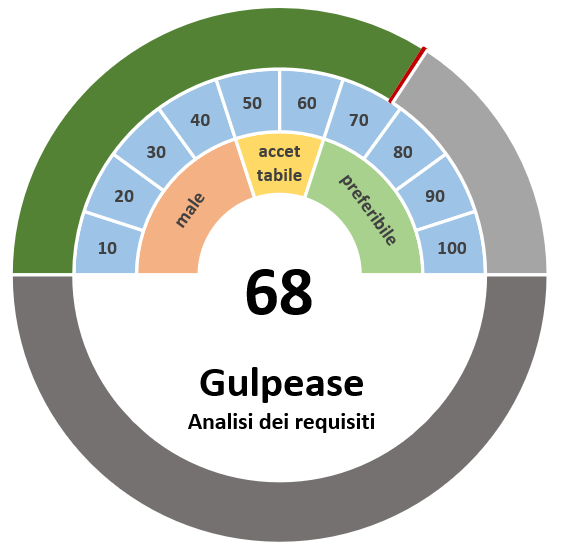
\includegraphics[width=\textwidth]{GulpeaseAdr.png}
        \caption{Gulpease di Analisi\_dei\_requisiti\_v1.0}
    \end{minipage}
    \hfill
    \begin{minipage}[b]{0.45\textwidth}
        \centering
        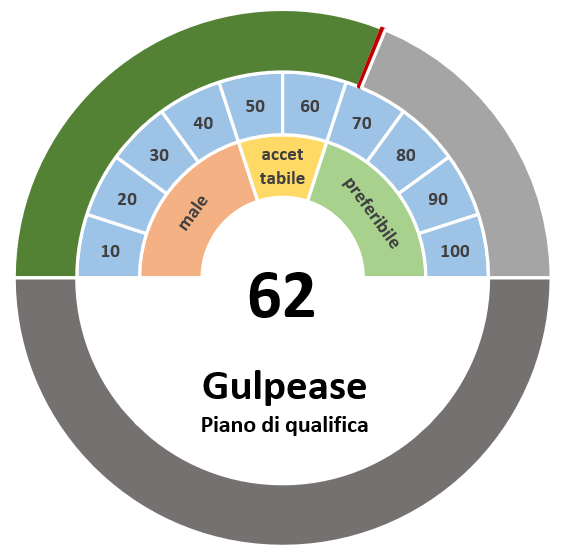
\includegraphics[width=\textwidth]{GulpeasePdq.png}
        \caption{Gulpease di Piano\_di\_qualifica\_v1.0}
    \end{minipage}
\end{figure}
\subsection{Analisi}
Analizzando i valori del cruscotto, è immediato notare che l'indice di ogni verbale è sempre stato superiore alla soglia di accettabilità. È inoltre utile notare che la maggior parte degli indici di Gulpease più bassi sono stati registrati in verbali esterni, mostrando come la natura più discorsiva di tali verbali mette a rischio maggiormente la leggibilità dei documenti.\\
L'elevata variabilità dei valori tra un documento e l'altro certifica la difficoltà nel migliorare tale metrica di qualità. Per questo motivo, è importante in futuro continuare a prestare attenzione alla struttura dei periodi delle frasi, in quanto un calo di attenzione porterebbe l'indice di un documento a non rispettare il valore di accettabilità.
